\chapter{Synthetic Controls}
\label{ch-syn-con}

This chapter is based on Refs.\cite{alves-book}
and \cite{book-mixtape}.

This chapter assumes that
the reader has read Chapter \ref{ch-did}
on the Difference-in-Differences (DID) method.

The Synthetic Controls (SC) method
is a simple enhancement of the DID method.
SC enhances DID in two simple
yet powerful ways:
\begin{enumerate}
\item{\bf Better time resolution.}
DID considers just 2 time-snapshots 
(i.e., a 
time-series with only 2 times)
whereas SC considers
arbitrarily many time-snapshots (i.e., a time-series with
more than 2 times).
\item{\bf Weighted average of controls.}
DID divides the population
of individuals into just 2 kinds:
the treated and the untreated (a.k.a. controls).
SC
divides the 
total population 
into treated and controls
just like DID does, but
it goes further and divides the control population into
multiple subpopulations,
and calculates a weighted average,
called a
``synthetic control",
of those subpopulations.
The weights of the synthetic
control are chosen so that
it mimics as closely as possible
the behavior
of  the treated population for all times
measured before the treatment
was applied.
\end{enumerate}


\begin{figure}[h!]
\centering
\includegraphics[width=3in]
{syn-con/syn-con-p-lines.png}
\caption{Pictorial
representation of the Synthetic Controls (SC) method.
The outcome $y$ of the synthetic control unit
is colored red and that of the treated unit
is colored blue.
They 
roughly agree for $t<t_*$.
} 
\label{fig-syn-con-p-lines}
\end{figure}

Let us describe these
two enhancements more precisely.

\begin{itemize}
\item{\bf timing}: 
Let $t_k$ for $k=0,1, \ldots, npre-1$
be the pre-treatment times at which
a measurement occurs. Let
$t_k$ for $k=npre, npre+1, \ldots, nt-1$
be the post-treatment times
at which a measurement occurs.
Note that
 $npre + npost=nt$. Note that
$t_*=t_{npre+1}$
is the first measurement time
after the treatment is applied,
$t_0$ is the first measurement time,
and $t_{fin}=t_{nt-1}$ is
the last one.

\item {\bf subpopulations}:
Let $S_1=\{\s_1\}$ be  the set of treated units
(just one). Let
$S_0 =\{\s:\s\neq \s_1\}$ be the
set of untreated units
 (i.e., controls).
Let $nsam=$ number of 
all units $\s$,
$n_1=|S_1|=1$, and
$n_0= |S_0|=nsam-1$.

\item{\bf weights}:

We want to define a
time-independent weight
$w^\s$ for each unit $\s$
in such a way
that the output $y^\s_t$
for the synthetic control
unit behaves like the 
output for the 
treated unit $\s_1$ for $t<t_*$.

Let
\beq
w^{\s_1}=0
\eeq
and

\beq
w^{n_0}=\{ w^\s\}_{\s\neq\s_1}
\;.
\eeq
Define a cost function $\calc$:
 
\beq
\calc(w^{n_0})=
\sum_{t<t_*}
\left(y^{\s_1}_t - \sum_{\s\neq \s_1}
w^\s y^\s_t\right)^2
\eeq
Then calculate $w^{n_0}$
by minimizing the cost function,
subject to the 
constraint that  $w^{n_0}$
be a probability distribution:

\beq
w^{n_0}=
\argmin_{W^{n_0}}
\left\{
\calc(W^{n_0}):
W^\s\geq 0, \sum_{\s\neq \s_1}W^\s =1
\right\}
\;.
\eeq
\end{itemize}
\hrule

Now that we have defined a weight $w^\s$
for every unit $\s$, we can define
for $c\in \bool$,

\beq
y^{\s_1}_t(c)=
\left\{
\begin{array}{ll}
y_t^{\s_1}&\text{ if } c=1
\\
\sum_{\s\neq \s_1}
w^\s y_t^\s&\text{ if } c=0
\end{array}
\right.
\eeq

\beq
\caly_c(t)=
E_\s[y_t^\s(c)]
\eeq
and

\beq
\delta_t= \caly_1(t)-\caly_0(t)
\eeq
$\delta_t$
is illustrated
in Fig.\ref{fig-syn-con-p-lines}.
It approximates $ATE(t)$.


\section{PO analysis}
In this section,
we show how
to analyze the
SC method
using the formalism of PO theory.



\begin{figure}[h!]
$$
\begin{array}{ccccc}
\xymatrix{
&\rvx\ar[dl]\ar[dr]
\\
\rvd\ar[rr]&&\rvy_t
}
&&
\xymatrix{
&&\rvx\ar[d]\ar[ddll]
\\
&&[\rvy_t(0), \rvy_t(1)]
\ar[d]
\\
\rvd\ar[rr]
&&\rvy_t
}
\\
\\
G_t&&G_{t, +}
\end{array}
$$
\caption{$t\in \{t_0, t_1, \ldots, 
t_{fin}\}$.
Bnet 
$G_{t,+}$
is obtained 
by adding
two new nodes
$\rvy_t(0)$
and $\rvy_t(1)$ to bnet $G_t$.}
\label{fig-syn-con-G-+}
\end{figure}

As usual for PO theory,
we will consider
expected values of $y^\s_t$:


\beq
E_{\s| d, x}[y^\s_t(c)]=
 E_{\rvy_t(c)| d, x}[\rvy_t(c)]=
\caly_{c| d, x}(t)
\eeq

To calculate these
expected values, we need a ``model"
with probability 
distributions.
In this case,
the needed model and probability
distributions are
provided by the
bnets depicted in Fig.\ref{fig-syn-con-G-+}.
The TPMs,
printed in blue,
for the 
 bnet
$G_{t, +}$
in Fig.\ref{fig-syn-con-G-+},
are as follows.
Note
that the
TPMs for the bnet $G_{t, +}$
are defined in 
terms
of the TPMs for the bnet $G_t$.



\beq\color{blue}
P(x)=P_{\rvx}(x)
\eeq

\beq\color{blue}
P(d|x)= 
P_{\rvd|\rvx}(d|x)
\eeq
 
\beq\color{blue}
P(y_t| y_t(0), y_t(1),d)=
\indi(y_t=y_t(d))
\eeq

\beq\color{blue}
P(y_t(c)|x)=
P(y_t(c)|d,x)=\text{given}
\eeq

\begin{figure}[h!]
\centering
\includegraphics[width=4in]
{syn-con/syn-con-bc.png}
\caption{Four different time-dependent
expected 
values $\caly_{c| d}(t)$ of $y^\s_t$
for bnet $G_{t, +}$
The $2*nt$ magenta  stars
represents the $2*nt$ SC measurements.} 
\label{fig-syn-con-bc}
\end{figure}




Fig.\ref{fig-syn-con-bc}
depicts the
four functions
$\caly_{c| d}(t)$
for $t$ in the interval  $[t_0, t_{fin}]$
and for $c, d\in \bool$.
The $\caly$ coordinates
of the $2*nt$ magenta stars in 
Fig.\ref{fig-syn-con-bc} can 
be calculated using bnet $G_t$.
Note that in Fig.\ref{fig-syn-con-bc},
we display a large gap
between the curves $\caly_{0| d}(t)$
for $ d\in \bool$.
In reality, $P(y_t(0)| d)$ has been
constructed so as to make that
gap as small as possible.
Thus, to a good(?) approximation,

\beq
\delta_t\approx ATE_t
\eeq
Unlike in the DID method,
in the SC method, to a good(?)
approximation, we don't have to worry
about parallel trends.